%% bare_jrnl_transmag.tex
%% V1.4b
%% 2015/08/26
%% by Michael Shell
%% see http://www.michaelshell.org/
%% for current contact information.
%%
%% This is a skeleton file demonstrating the use of IEEEtran.cls
%% (requires IEEEtran.cls version 1.8b or later) with an IEEE 
%% Transactions on Magnetics journal paper.
%%
%% Support sites:
%% http://www.michaelshell.org/tex/ieeetran/
%% http://www.ctan.org/pkg/ieeetran
%% and
%% http://www.ieee.org/

%%*************************************************************************
%% Legal Notice:
%% This code is offered as-is without any warranty either expressed or
%% implied; without even the implied warranty of MERCHANTABILITY or
%% FITNESS FOR A PARTICULAR PURPOSE! 
%% User assumes all risk.
%% In no event shall the IEEE or any contributor to this code be liable for
%% any damages or losses, including, but not limited to, incidental,
%% consequential, or any other damages, resulting from the use or misuse
%% of any information contained here.
%%
%% All comments are the opinions of their respective authors and are not
%% necessarily endorsed by the IEEE.
%%
%% This work is distributed under the LaTeX Project Public License (LPPL)
%% ( http://www.latex-project.org/ ) version 1.3, and may be freely used,
%% distributed and modified. A copy of the LPPL, version 1.3, is included
%% in the base LaTeX documentation of all distributions of LaTeX released
%% 2003/12/01 or later.
%% Retain all contribution notices and credits.
%% ** Modified files should be clearly indicated as such, including  **
%% ** renaming them and changing author support contact information. **
%%*************************************************************************


% *** Authors should verify (and, if needed, correct) their LaTeX system  ***
% *** with the testflow diagnostic prior to trusting their LaTeX platform ***
% *** with production work. The IEEE's font choices and paper sizes can   ***
% *** trigger bugs that do not appear when using other class files.       ***                          ***
% The testflow support page is at:
% http://www.michaelshell.org/tex/testflow/



\documentclass[journal,transmag]{IEEEtran}
%
% If IEEEtran.cls has not been installed into the LaTeX system files,
% manually specify the path to it like:
% \documentclass[journal]{../sty/IEEEtran}





% Some very useful LaTeX packages include:
% (uncomment the ones you want to load)


% *** MISC UTILITY PACKAGES ***
%
%\usepackage{ifpdf}
% Heiko Oberdiek's ifpdf.sty is very useful if you need conditional
% compilation based on whether the output is pdf or dvi.
% usage:
% \ifpdf
%   % pdf code
% \else
%   % dvi code
% \fi
% The latest version of ifpdf.sty can be obtained from:
% http://www.ctan.org/pkg/ifpdf
% Also, note that IEEEtran.cls V1.7 and later provides a builtin
% \ifCLASSINFOpdf conditional that works the same way.
% When switching from latex to pdflatex and vice-versa, the compiler may
% have to be run twice to clear warning/error messages.






% *** CITATION PACKAGES ***
%
%\usepackage{cite}
% cite.sty was written by Donald Arseneau
% V1.6 and later of IEEEtran pre-defines the format of the cite.sty package
% \cite{} output to follow that of the IEEE. Loading the cite package will
% result in citation numbers being automatically sorted and properly
% "compressed/ranged". e.g., [1], [9], [2], [7], [5], [6] without using
% cite.sty will become [1], [2], [5]--[7], [9] using cite.sty. cite.sty's
% \cite will automatically add leading space, if needed. Use cite.sty's
% noadjust option (cite.sty V3.8 and later) if you want to turn this off
% such as if a citation ever needs to be enclosed in parenthesis.
% cite.sty is already installed on most LaTeX systems. Be sure and use
% version 5.0 (2009-03-20) and later if using hyperref.sty.
% The latest version can be obtained at:
% http://www.ctan.org/pkg/cite
% The documentation is contained in the cite.sty file itself.






% *** GRAPHICS RELATED PACKAGES ***
%
\ifCLASSINFOpdf
  % \usepackage[pdftex]{graphicx}
  % declare the path(s) where your graphic files are
  % \graphicspath{{../pdf/}{../jpeg/}}
  % and their extensions so you won't have to specify these with
  % every instance of \includegraphics
  % \DeclareGraphicsExtensions{.pdf,.jpeg,.png}
\else
  % or other class option (dvipsone, dvipdf, if not using dvips). graphicx
  % will default to the driver specified in the system graphics.cfg if no
  % driver is specified.
  % \usepackage[dvips]{graphicx}
  % declare the path(s) where your graphic files are
  % \graphicspath{{../eps/}}
  % and their extensions so you won't have to specify these with
  % every instance of \includegraphics
  % \DeclareGraphicsExtensions{.eps}
\fi
% graphicx was written by David Carlisle and Sebastian Rahtz. It is
% required if you want graphics, photos, etc. graphicx.sty is already
% installed on most LaTeX systems. The latest version and documentation
% can be obtained at: 
% http://www.ctan.org/pkg/graphicx
% Another good source of documentation is "Using Imported Graphics in
% LaTeX2e" by Keith Reckdahl which can be found at:
% http://www.ctan.org/pkg/epslatex
%
% latex, and pdflatex in dvi mode, support graphics in encapsulated
% postscript (.eps) format. pdflatex in pdf mode supports graphics
% in .pdf, .jpeg, .png and .mps (metapost) formats. Users should ensure
% that all non-photo figures use a vector format (.eps, .pdf, .mps) and
% not a bitmapped formats (.jpeg, .png). The IEEE frowns on bitmapped formats
% which can result in "jaggedy"/blurry rendering of lines and letters as
% well as large increases in file sizes.
%
% You can find documentation about the pdfTeX application at:
% http://www.tug.org/applications/pdftex




% *** MATH PACKAGES ***
%
%\usepackage{amsmath}
% A popular package from the American Mathematical Society that provides
% many useful and powerful commands for dealing with mathematics.
%
% Note that the amsmath package sets \interdisplaylinepenalty to 10000
% thus preventing page breaks from occurring within multiline equations. Use:
%\interdisplaylinepenalty=2500
% after loading amsmath to restore such page breaks as IEEEtran.cls normally
% does. amsmath.sty is already installed on most LaTeX systems. The latest
% version and documentation can be obtained at:
% http://www.ctan.org/pkg/amsmath





% *** SPECIALIZED LIST PACKAGES ***
%
%\usepackage{algorithmic}
% algorithmic.sty was written by Peter Williams and Rogerio Brito.
% This package provides an algorithmic environment fo describing algorithms.
% You can use the algorithmic environment in-text or within a figure
% environment to provide for a floating algorithm. Do NOT use the algorithm
% floating environment provided by algorithm.sty (by the same authors) or
% algorithm2e.sty (by Christophe Fiorio) as the IEEE does not use dedicated
% algorithm float types and packages that provide these will not provide
% correct IEEE style captions. The latest version and documentation of
% algorithmic.sty can be obtained at:
% http://www.ctan.org/pkg/algorithms
% Also of interest may be the (relatively newer and more customizable)
% algorithmicx.sty package by Szasz Janos:
% http://www.ctan.org/pkg/algorithmicx




% *** ALIGNMENT PACKAGES ***
%
%\usepackage{array}
% Frank Mittelbach's and David Carlisle's array.sty patches and improves
% the standard LaTeX2e array and tabular environments to provide better
% appearance and additional user controls. As the default LaTeX2e table
% generation code is lacking to the point of almost being broken with
% respect to the quality of the end results, all users are strongly
% advised to use an enhanced (at the very least that provided by array.sty)
% set of table tools. array.sty is already installed on most systems. The
% latest version and documentation can be obtained at:
% http://www.ctan.org/pkg/array


% IEEEtran contains the IEEEeqnarray family of commands that can be used to
% generate multiline equations as well as matrices, tables, etc., of high
% quality.




% *** SUBFIGURE PACKAGES ***
%\ifCLASSOPTIONcompsoc
%  \usepackage[caption=false,font=normalsize,labelfont=sf,textfont=sf]{subfig}
%\else
%  \usepackage[caption=false,font=footnotesize]{subfig}
%\fi
% subfig.sty, written by Steven Douglas Cochran, is the modern replacement
% for subfigure.sty, the latter of which is no longer maintained and is
% incompatible with some LaTeX packages including fixltx2e. However,
% subfig.sty requires and automatically loads Axel Sommerfeldt's caption.sty
% which will override IEEEtran.cls' handling of captions and this will result
% in non-IEEE style figure/table captions. To prevent this problem, be sure
% and invoke subfig.sty's "caption=false" package option (available since
% subfig.sty version 1.3, 2005/06/28) as this is will preserve IEEEtran.cls
% handling of captions.
% Note that the Computer Society format requires a larger sans serif font
% than the serif footnote size font used in traditional IEEE formatting
% and thus the need to invoke different subfig.sty package options depending
% on whether compsoc mode has been enabled.
%
% The latest version and documentation of subfig.sty can be obtained at:
% http://www.ctan.org/pkg/subfig



% *** FLOAT PACKAGES ***
%
%\usepackage{fixltx2e}
% fixltx2e, the successor to the earlier fix2col.sty, was written by
% Frank Mittelbach and David Carlisle. This package corrects a few problems
% in the LaTeX2e kernel, the most notable of which is that in current
% LaTeX2e releases, the ordering of single and double column floats is not
% guaranteed to be preserved. Thus, an unpatched LaTeX2e can allow a
% single column figure to be placed prior to an earlier double column
% figure.
% Be aware that LaTeX2e kernels dated 2015 and later have fixltx2e.sty's
% corrections already built into the system in which case a warning will
% be issued if an attempt is made to load fixltx2e.sty as it is no longer
% needed.
% The latest version and documentation can be found at:
% http://www.ctan.org/pkg/fixltx2e


%\usepackage{stfloats}
% stfloats.sty was written by Sigitas Tolusis. This package gives LaTeX2e
% the ability to do double column floats at the bottom of the page as well
% as the top. (e.g., "\begin{figure*}[!b]" is not normally possible in
% LaTeX2e). It also provides a command:
%\fnbelowfloat
% to enable the placement of footnotes below bottom floats (the standard
% LaTeX2e kernel puts them above bottom floats). This is an invasive package
% which rewrites many portions of the LaTeX2e float routines. It may not work
% with other packages that modify the LaTeX2e float routines. The latest
% version and documentation can be obtained at:
% http://www.ctan.org/pkg/stfloats
% Do not use the stfloats baselinefloat ability as the IEEE does not allow
% \baselineskip to stretch. Authors submitting work to the IEEE should note
% that the IEEE rarely uses double column equations and that authors should try
% to avoid such use. Do not be tempted to use the cuted.sty or midfloat.sty
% packages (also by Sigitas Tolusis) as the IEEE does not format its papers in
% such ways.
% Do not attempt to use stfloats with fixltx2e as they are incompatible.
% Instead, use Morten Hogholm'a dblfloatfix which combines the features
% of both fixltx2e and stfloats:
%
% \usepackage{dblfloatfix}
% The latest version can be found at:
% http://www.ctan.org/pkg/dblfloatfix




%\ifCLASSOPTIONcaptionsoff
%  \usepackage[nomarkers]{endfloat}
% \let\MYoriglatexcaption\caption
% \renewcommand{\caption}[2][\relax]{\MYoriglatexcaption[#2]{#2}}
%\fi
% endfloat.sty was written by James Darrell McCauley, Jeff Goldberg and 
% Axel Sommerfeldt. This package may be useful when used in conjunction with 
% IEEEtran.cls'  captionsoff option. Some IEEE journals/societies require that
% submissions have lists of figures/tables at the end of the paper and that
% figures/tables without any captions are placed on a page by themselves at
% the end of the document. If needed, the draftcls IEEEtran class option or
% \CLASSINPUTbaselinestretch interface can be used to increase the line
% spacing as well. Be sure and use the nomarkers option of endfloat to
% prevent endfloat from "marking" where the figures would have been placed
% in the text. The two hack lines of code above are a slight modification of
% that suggested by in the endfloat docs (section 8.4.1) to ensure that
% the full captions always appear in the list of figures/tables - even if
% the user used the short optional argument of \caption[]{}.
% IEEE papers do not typically make use of \caption[]'s optional argument,
% so this should not be an issue. A similar trick can be used to disable
% captions of packages such as subfig.sty that lack options to turn off
% the subcaptions:
% For subfig.sty:
% \let\MYorigsubfloat\subfloat
% \renewcommand{\subfloat}[2][\relax]{\MYorigsubfloat[]{#2}}
% However, the above trick will not work if both optional arguments of
% the \subfloat command are used. Furthermore, there needs to be a
% description of each subfigure *somewhere* and endfloat does not add
% subfigure captions to its list of figures. Thus, the best approach is to
% avoid the use of subfigure captions (many IEEE journals avoid them anyway)
% and instead reference/explain all the subfigures within the main caption.
% The latest version of endfloat.sty and its documentation can obtained at:
% http://www.ctan.org/pkg/endfloat
%
% The IEEEtran \ifCLASSOPTIONcaptionsoff conditional can also be used
% later in the document, say, to conditionally put the References on a 
% page by themselves.




% *** PDF, URL AND HYPERLINK PACKAGES ***
%
%\usepackage{url}
% url.sty was written by Donald Arseneau. It provides better support for
% handling and breaking URLs. url.sty is already installed on most LaTeX
% systems. The latest version and documentation can be obtained at:
% http://www.ctan.org/pkg/url
% Basically, \url{my_url_here}.




% *** Do not adjust lengths that control margins, column widths, etc. ***
% *** Do not use packages that alter fonts (such as pslatex).         ***
% There should be no need to do such things with IEEEtran.cls V1.6 and later.
% (Unless specifically asked to do so by the journal or conference you plan
% to submit to, of course. )

\usepackage{amsmath}
\usepackage{subcaption}
\usepackage{graphicx}
\usepackage{url}
\usepackage{array}
\usepackage{algorithm}
\usepackage{algorithmic}
\usepackage{multicol}
\usepackage[skip=0pt]{caption} 
\usepackage{float}


\begin{document}
%
% paper title
% Titles are generally capitalized except for words such as a, an, and, as,
% at, but, by, for, in, nor, of, on, or, the, to and up, which are usually
% not capitalized unless they are the first or last word of the title.
% Linebreaks \\ can be used within to get better formatting as desired.
% Do not put math or special symbols in the title.
\title{\textbf{SmartCamera Module} \\ \textit{Innovating Self-Learning Software for Intelligent Vision}}



% author names and affiliations
% transmag papers use the long conference author name format.

\author{\IEEEauthorblockN{SangWoo Park,
Hantao Fu},
\IEEEauthorblockA{Electrical \& Computer Engineering, Rice University, Houston, TX 77005 USA}

%\thanks{Revised Mar 24,2025. Author:SangWoo.P}
}



% The paper headers
\markboth{Y25 ELEC594}%
{Shell \MakeLowercase{\textit{et al.}}: SmartCam Module}
% The only time the second header will appear is for the odd numbered pages
% after the title page when using the twoside option.
% 
% *** Note that you probably will NOT want to include the author's ***
% *** name in the headers of peer review papers.                   ***
% You can use \ifCLASSOPTIONpeerreview for conditional compilation here if
% you desire.




% If you want to put a publisher's ID mark on the page you can do it like
% this:
%\IEEEpubid{0000--0000/00\$00.00~\copyright~2015 IEEE}
% Remember, if you use this you must call \IEEEpubidadjcol in the second
% column for its text to clear the IEEEpubid mark.



% use for special paper notices
%\IEEEspecialpapernotice{(Invited Paper)}


% for Transactions on Magnetics papers, we must declare the abstract and
% index terms PRIOR to the title within the \IEEEtitleabstractindextext
% IEEEtran command as these need to go into the title area created by
% \maketitle.
% As a general rule, do not put math, special symbols or citations
% in the abstract or keywords.
\IEEEtitleabstractindextext{%
\begin{abstract}
In this project, KTM Technology aims to expand into the professional camera module sector by developing an integrated training module that combines hardware and software to optimize costs. To achieve this, we plan to develop a training software for camera modules capable of learning from real-world data under various conditions.Through our initial research, we have identified seven key solutions that provide valuable insights into industry approaches [1]–[7]. Inspired by these references, we will further explore and refine more frameworks to guide our development. Our proposed solution will build on existing methodologies across various fields, including drones, medical devices, and material characterization equipment, while incorporating enhanced features to improve performance and versatility.The primary goal for this semester is to implement our training software into commercially available camera hardware, enabling it to identify specific objects with reasonable accuracy. Our focus will be on establishing a robust framework for the camera module, while aspects such as stability, error minimization, and seamless functionality will be addressed in the following semester.
\end{abstract}

% Note that keywords are not normally used for peerreview papers.
\begin{IEEEkeywords}
Camera Vision, AI, Training module, Big data, Machine learning, ADAS, Autonomous driving, Automotive.
\end{IEEEkeywords}}



% make the title area
\maketitle


% To allow for easy dual compilation without having to reenter the
% abstract/keywords data, the \IEEEtitleabstractindextext text will
% not be used in maketitle, but will appear (i.e., to be "transported")
% here as \IEEEdisplaynontitleabstractindextext when the compsoc 
% or transmag modes are not selected <OR> if conference mode is selected 
% - because all conference papers position the abstract like regular
% papers do.
\IEEEdisplaynontitleabstractindextext
% \IEEEdisplaynontitleabstractindextext has no effect when using
% compsoc or transmag under a non-conference mode.







% For peer review papers, you can put extra information on the cover
% page as needed:
% \ifCLASSOPTIONpeerreview
% \begin{center} \bfseries EDICS Category: 3-BBND \end{center}
% \fi
%
% For peerreview papers, this IEEEtran command inserts a page break and
% creates the second title. It will be ignored for other modes.
%\IEEEpeerreviewmaketitle



\section{Introduction}
% The very first letter is a 2 line initial drop letter followed
% by the rest of the first word in caps.
% 
% form to use if the first word consists of a single letter:
% \IEEEPARstart{A}{demo} file is ....
% 
% form to use if you need the single drop letter followed by
% normal text (unknown if ever used by the IEEE):
% \IEEEPARstart{A}{}demo file is ....
% 
% Some journals put the first two words in caps:
% \IEEEPARstart{T}{his demo} file is ....
% 
% Here we have the typical use of a "T" for an initial drop letter
% and "HIS" in caps to complete the first word.


%\subsection{Background \& Industry Relevance}
\IEEEPARstart
The rapid advancement of electric vehicles has intensified the demand for high-performance vision systems capable of real-time environmental perception and decision making. As automotive manufacturers integrate sophisticated driver-assistance and autonomous navigation technologies, intelligent camera modules must evolve beyond static recognition models to incorporate dynamic learning capabilities. Current market solutions on camera modules are shown in Table ~\ref{tab:Current_Market_Products}

This project seeks to develop an advanced AI-driven training module for camera systems, aiming to develop a camera module that closely approaches the performance of commonly available commercial products. Building on these studies, this project will advance AI-driven camera module capabilities by integrating adaptive training frameworks that enhance recognition performance, computational efficiency, and real-world deployability.


\begin{table*}[t]
\centering
\caption{Main Camera Module Providers for Autonomous Driving}
\label{tab:Current_Market_Products}
\begin{tabular}{|c|p{6.5cm}|p{5.5cm}|}  
\hline
\textbf{Manufacturer} & \textbf{Core Technology / Product} & \textbf{Major Automotive Partners} \\
\hline
Mobileye & EyeQ + Multi-camera System & NIO, Ford, etc. \\
\hline
Tesla & Tesla Vision (Vision-only System) & In-house Integration \\
\hline
Sony & IMX Series Image Sensors & Multiple OEM Partnerships \\
\hline
Valeo & Night Vision + Surround View System & BMW, Mercedes-Benz, etc. \\
\hline
NVIDIA & Hyperion Platform & Various Robotaxi Manufacturers \\
\hline
Aptiv & ADAS Camera Modules & Volkswagen, Hyundai, etc. \\
\hline
\end{tabular}
\end{table*}


% You must have at least 2 lines in the paragraph with the drop letter
% (should never be an issue)




\section{Methodology}
Our approach is divided into 2 main components, as shown in Fig.~\ref{fig:The Structure of our Approach}, including software module and hardware module. Such a modular designing style makes the project more organized and facilitates future debugging and improvement.

\begin{figure}[h]
    \centering
    \includegraphics[width=0.5\textwidth]{The Structure of our Approach.png} 
    \caption{The Structure of our Approach}
    \label{fig:The Structure of our Approach}
\end{figure}

\subsection{Software Module}

In this project, we divide the whole software module into 3 parts, including data acquisition, data processing and decision making, as shown in Table~\ref{tab:Software Module of our Smart Camera System}. 

i. \textbf{Data Acquisition: }The data acquisition module is responsible for rapidly and accurately identifying specific objects within the camera’s field of view. The algorithms applied at this stage must be both sensitive and robust, capable of detecting target features within milliseconds. This ensures that the system captures relevant visual data in real time, forming the foundation for subsequent analysis and decision-making. Representative algorithms for this stage include YOLOv8, SSD (Single Shot MultiBox Detector), and Faster R-CNN, all of which are widely used for real-time object detection tasks.

ii. \textbf{Data Processing: }The data processing module further analyzes the raw data obtained from the acquisition stage. Its primary task is to extract key physical characteristics of each identified object, including size, shape, color, and relative distance. These parameters provide essential context for interpreting the environment and evaluating potential risks or navigational considerations. Representative algorithms include keypoint detection (e.g., OpenPose), segmentation networks such as Mask R-CNN, and depth estimation models like MiDaS.

iii. \textbf{Decision Making: } The decision-making module interprets the outputs from the previous two stages and generates appropriate responses for the vehicle. Based on the identified objects and their characteristics, this module determines whether the system should trigger braking, acceleration, steering adjustments, or other driving actions. Its effectiveness directly impacts the overall safety and performance of the autonomous system. Representative algorithms for this layer include finite state machines (FSM), reinforcement learning-based policy networks, and behavior cloning models trained from expert demonstrations.

\begin{table*}[t]
\centering
\caption{Software Module of our Smart Camera System}
\label{tab:Software Module of our Smart Camera System}
\begin{tabular}{|c|p{7.5cm}|p{5.5cm}|}  
\hline
\textbf{Level} & \textbf{Key Properties} & \textbf{Representative Algorithms} \\
\hline
Data Acquisition & High sensitivity, strong robustness, millisecond-level response, rapid detection of image targets & YOLOv8, SSD, Faster R-CNN \\
\hline
Data Processing & Accurately extract physical features such as \textbf{size}, \textbf{shape}, \textbf{color}, and \textbf{distance} & OpenPose, Mask R-CNN, MiDaS \\
\hline
Decision Making & Make \textbf{real-time decisions} based on analysis results and generate control commands (e.g., braking, acceleration, steering) & FSM (Finite State Machine), Reinforcement Learning, Behavior Cloning \\
\hline
\end{tabular}
\end{table*}

\subsection{Hardware Module}
We divide the whole module into 3 parts, including hardware selection, hardware assembly, and hardware operation. 

i. \textbf{Hardware Selection: }In this step, we evaluate the hardware platforms that best support our trained AI models, considering constraints such as processing power, memory capacity, compatibility with camera interfaces, and real-time performance. Typical choices include devices like Raspberry Pi, Jetson Nano, or other ARM-based edge computing platforms.

ii. \textbf{Hardware Assembly: }This phase involves integrating selected hardware components—such as camera modules, processing units, and connectors—into a functional unit. Emphasis is placed on stability, connectivity, and ease of deployment, ensuring that the hardware can operate reliably under dynamic driving conditions.

iii. \textbf{Hardware Operation: } After successful assembly, we deploy the trained software to the embedded hardware and test the complete system in real-time scenarios. This step helps identify mismatches between simulated and real-world performance and improves deployment reliability through iterative debugging and tuning.


\section{Experiment}
\subsection{Algorithm Selecting}
During this semester, our efforts were primarily dedicated to the data acquisition component of the software module, for which we adopted YOLOv8 as the core detection algorithm.

YOLO (You Look Only Once) is a state-of-the-art deep learning model known for its real-time speed, high accuracy, and computational efficiency. Unlike two-stage detectors like Faster R-CNN, YOLO follows a single-stage framework, processing an entire image in one forward pass to perform classification and localization simultaneously. This eliminates the need for region proposals, significantly reducing computational overhead. Its working architecture are demonstrated in Fig.~\ref{fig:external_yolo} [8]:

i. \textbf{Image Preprocessing: } The input image is resized to a fixed dimension (e.g., 416 × 416 or 608 × 608) and normalized to enhance computational efficiency. The resized image is then passed through a CNN backbone for feature extraction.


ii. \textbf{Grid-Based Localization: } The image is divided into an $S \times S$ grid, where each grid cell is responsible for detecting objects whose centers fall within it. Each cell predicts multiple bounding boxes, along with confidence scores and class probabilities.

iii. \textbf{Bounding Box Prediction: } Each grid cell predicts $B$ bounding boxes, where each bounding box consists of:
\begin{itemize}
  \setlength{\itemindent}{1em} 
  \item $(x, y)$: The center coordinates relative to the grid cell.
  \item $(w, h)$: The width and height normalized to the entire image.
  \item Confidence score: The likelihood that the bounding box contains an object.
  \item Class probabilities: The probability distribution over predefined object categories.
\end{itemize}

iv. \textbf{Non-Maximum Suppression: } To eliminate redundant bounding boxes, YOLO employs Non-Maximum Suppression \textbf{(NMS)}, which:
\begin{itemize}
  \setlength{\itemindent}{2em} 
  \item Selects the bounding box with the highest confidence score.
  \item Removes overlapping boxes with an Intersection over Union \textbf{(IoU)} threshold (e.g., 0.5).
  \item Retains only the most relevant bounding boxes.
\end{itemize}

\begin{figure}[h]
    \centering
    \includegraphics[width=0.45\textwidth]{YOLO.png}
    \caption{YOLO's Working Architecture. Source: [8]}
    \label{fig:external_yolo}
\end{figure}

\subsection{Model Training}

The process of training an object detection model with the YOLOv8 algorithm consists of three key stages: preparing the dataset, developing the training script, and executing the training process.\\

i. \textbf{Preparing the Dataset: } 

Datasets for training YOLOv8 models generally come from two main sources. The first includes publicly available open-source datasets, which can be downloaded from platforms such as COCO or Roboflow. The second involves custom-built datasets, created by manually annotating raw images using tools like LabelImg, which then generate annotation files in a format compatible with the YOLOv8 algorithm. During this semester, we primarily utilized publicly available datasets as the main source of training data for the YOLOv8 model.

To ensure that YOLOv8 can correctly associate each image with its corresponding label during training, the dataset must follow a standardized structure, as shown in Fig.~\ref{fig:Structure of Dataset}. 

\begin{figure}[h]
    \centering
    \includegraphics[width=0.3\textwidth]{Structure of Dataset.png}
    \caption{Structure of Dataset}
    \label{fig:Structure of Dataset}
\end{figure}

In the first-level directory, the train directory contains images used for training models by updating its weights and parameters through backpropagation, the valid directory stores images for detecting model's performance in real time when training, the test directory is primarily used for evaluating model's generalization ability through images not used by the train and valid directories, and the data.yaml is placed at the root of the dataset, specifying the training and validation image paths, number of classes, and class names.

In the second-level directory, the images directory contains all image files, while labels directory mirrors the structure of images, containing a .txt annotation file for each image. \\

ii. \textbf{Developing the Training Script} 

Since the tools for training YOLOv8 models are fully integrated within the \textit{ultralytics} library, our training script is highly streamlined, with a clear logical structure and minimal code complexity. The logic of YOLOv8 Training Script can be checked at Algorithm 1 in Appendix. 

The \textit{yolov8n.pt} here is a pre-trained model from the YOLOv8-nano family trained on the COCO dataset. It offers a strong initialization that accelerates convergence and improves accuracy, which means that we are able to pursue higher performance for our YOLOv8 model by using less training datasets. 

The \textit{data.yaml} here serves as a configuration  interface that defines essential parameters for model training. It specifies the paths to the training, validation, and optional test datasets, along with the total number of classes (nc) and the list of class names (names). By referencing this file, the YOLO training script can automatically load the corresponding images and labels, making data.yaml a critical bridge between the dataset and the model.\\


iii. \textbf{Executing the Training Process} 

Upon running the training script, two key weight files are generated: \textit{best.pt} and \textit{last.pt}. The \textit{best.pt} file stores the model parameters that achieved the highest performance on the validation set throughout the training process, typically determined by the maximum mean Average Precision (mAP). It is considered the most reliable version for inference, deployment, or model export. On the other hand, \textit{last.pt} captures the model’s state after the final training epoch. While it may not yield the best validation results, it is useful for resuming training or conducting performance comparisons across epochs. 

\subsection{Model Testing}
In this experiment, we use \textit{best.pt} as the ultimate YOLOv8 model, which will be used to conduct object detection in images, videos and real-time recording. 

i. \textbf{Image Scenario:} In this scenario, we plan to collect images from various online platforms and apply the best.pt model to perform object detection, aiming to evaluate the model’s effectiveness in diverse visual contexts. The logic of Image Scenario Testing Code can be checked at Algorithm 2 in Appendix.


ii. \textbf{Video Scenario:} In this scenario, we plan to collect videos from various online platforms, particularly dashcam footage, and apply the best.pt model to perform object detection in real time as the video plays, in order to assess the model’s detection performance under dynamic conditions.The Logic of Video Scenario Testing Code can be found at Algorithm 3 in Appendix.


iii. \textbf{Real-time Recording Scenario:} In this scenario, we plan to utilize an external camera connected via USB to capture the surrounding environment in real time. The best.pt model will be applied during the live video stream to perform real-time object detection, allowing us to assess the model’s performance under practical, dynamic conditions.The Logic of Real-time Recording Scenario Testing Code can be found at Algorithm 4 in Appendix.


\section{Results}


\subsection{Result of Image Scenario}

i. \textbf{System Efficiency \& Computational Bench-marking:}

In the midterm report, we evaluated the performance of a publicly available model from GitHub using a set of test images. At this stage, we reuse the same image set to compare results and highlight the improved performance of our own trained model.

As shown in Fig~\ref{fig:Image Scenario 1}, compared to model in mid-term report, the current one improves its average confidence score. 

\begin{figure}[h]
    \centering
    \begin{subfigure}[b]{0.225\textwidth}
        \includegraphics[width=\textwidth]{Result_1.png}
        \caption{Performance of the mid-term model}
        \label{fig:Result_1}
    \end{subfigure}
    \hfill
    \begin{subfigure}[b]{0.225\textwidth}
        \includegraphics[width=\textwidth]{Result_1_new.jpg}
        \caption{Performance of the current model
}
        \label{fig:Result_1_new}
    \end{subfigure}
    \caption{Image Scenario 1}
    \label{fig:Image Scenario 1}
\end{figure}

As shown in Fig~\ref{fig:Image Scenario 2}, compared to model in mid-term report, the current one are able to detect horizontally oriented traffic lights with relatively high confidence score. 

\begin{figure}[h]
    \centering
    \begin{subfigure}[b]{0.225\textwidth}
        \includegraphics[width=\textwidth]{Result_2.png}
        \caption{Performance of the mid-term model}
        \label{fig:Result_2}
    \end{subfigure}
    \hfill
    \begin{subfigure}[b]{0.225\textwidth}
        \includegraphics[width=\textwidth]{Result_2_new.jpg}
        \caption{Performance of the current model
}
        \label{fig:Result_2_new}
    \end{subfigure}
    \caption{Image Scenario 2}
    \label{fig:Image Scenario 2}
\end{figure}

As shown in Fig~\ref{fig:Image Scenario 3}, compared to model in mid-term report, the current one works much better with relatively high confidence scores when traffic Lights are too close or too far 

\begin{figure}[h]
    \centering
    \begin{subfigure}[b]{0.225\textwidth}
        \includegraphics[width=\textwidth]{Result_3.png}
        \caption{Performance of the mid-term model}
        \label{fig:Result_3}
    \end{subfigure}
    \hfill
    \begin{subfigure}[b]{0.225\textwidth}
        \includegraphics[width=\textwidth]{Result_3_new.jpg}
        \caption{Performance of the current model
}
        \label{fig:Result_3_new}
    \end{subfigure}
    \caption{Image Scenario 3}
    \label{fig:Image Scenario 3}
\end{figure}

ii. \textbf{Observed Limitations \& Failure Cases:}

As shown in Fig.~\ref{fig:Image Scenario 1}, the current model consistently fails to exceed a confidence score of 0.85, indicating limitations in its detection reliability.

As shown in Fig.~\ref{fig:Image Scenario 2}, the current model occasionally misses certain objects, such as the traffic light located at the far left of the image.

As shown in Fig.~\ref{fig:Image Scenario 4}, the current model still lacks the capability to interpret the orientation of traffic lights, as evidenced by its failure to recognize the direction of the traffic light on the far left of the image.

\begin{figure}[h]
    \centering
    \begin{subfigure}[b]{0.225\textwidth}
        \includegraphics[width=\textwidth]{Result_4.png}
        \caption{Performance of the mid-term model}
        \label{fig:Result_4}
    \end{subfigure}
    \hfill
    \begin{subfigure}[b]{0.225\textwidth}
        \includegraphics[width=\textwidth]{Result_4_new.jpg}
        \caption{Performance of the current model
}
        \label{fig:Result_4_new}
    \end{subfigure}
    \caption{Image Scenario 3}
    \label{fig:Image Scenario 4}
\end{figure}

\subsection{Result of Video Scenario}

i. \textbf{System Efficiency \& Computational Bench-marking:}

As shown in Fig.~\ref{fig:Video Scenario 1}, the model used in the midterm report was limited to traffic light detection and exhibited subpar performance, resulting in unsatisfactory outcomes in the video scenario. In contrast, the current model—enhanced through exposure to a larger dataset and multiple training iterations—has begun to demonstrate the fundamental object detection capabilities expected of an onboard intelligent camera in autonomous vehicles.

\begin{figure}[h]
    \centering
    \begin{subfigure}[b]{0.225\textwidth}
        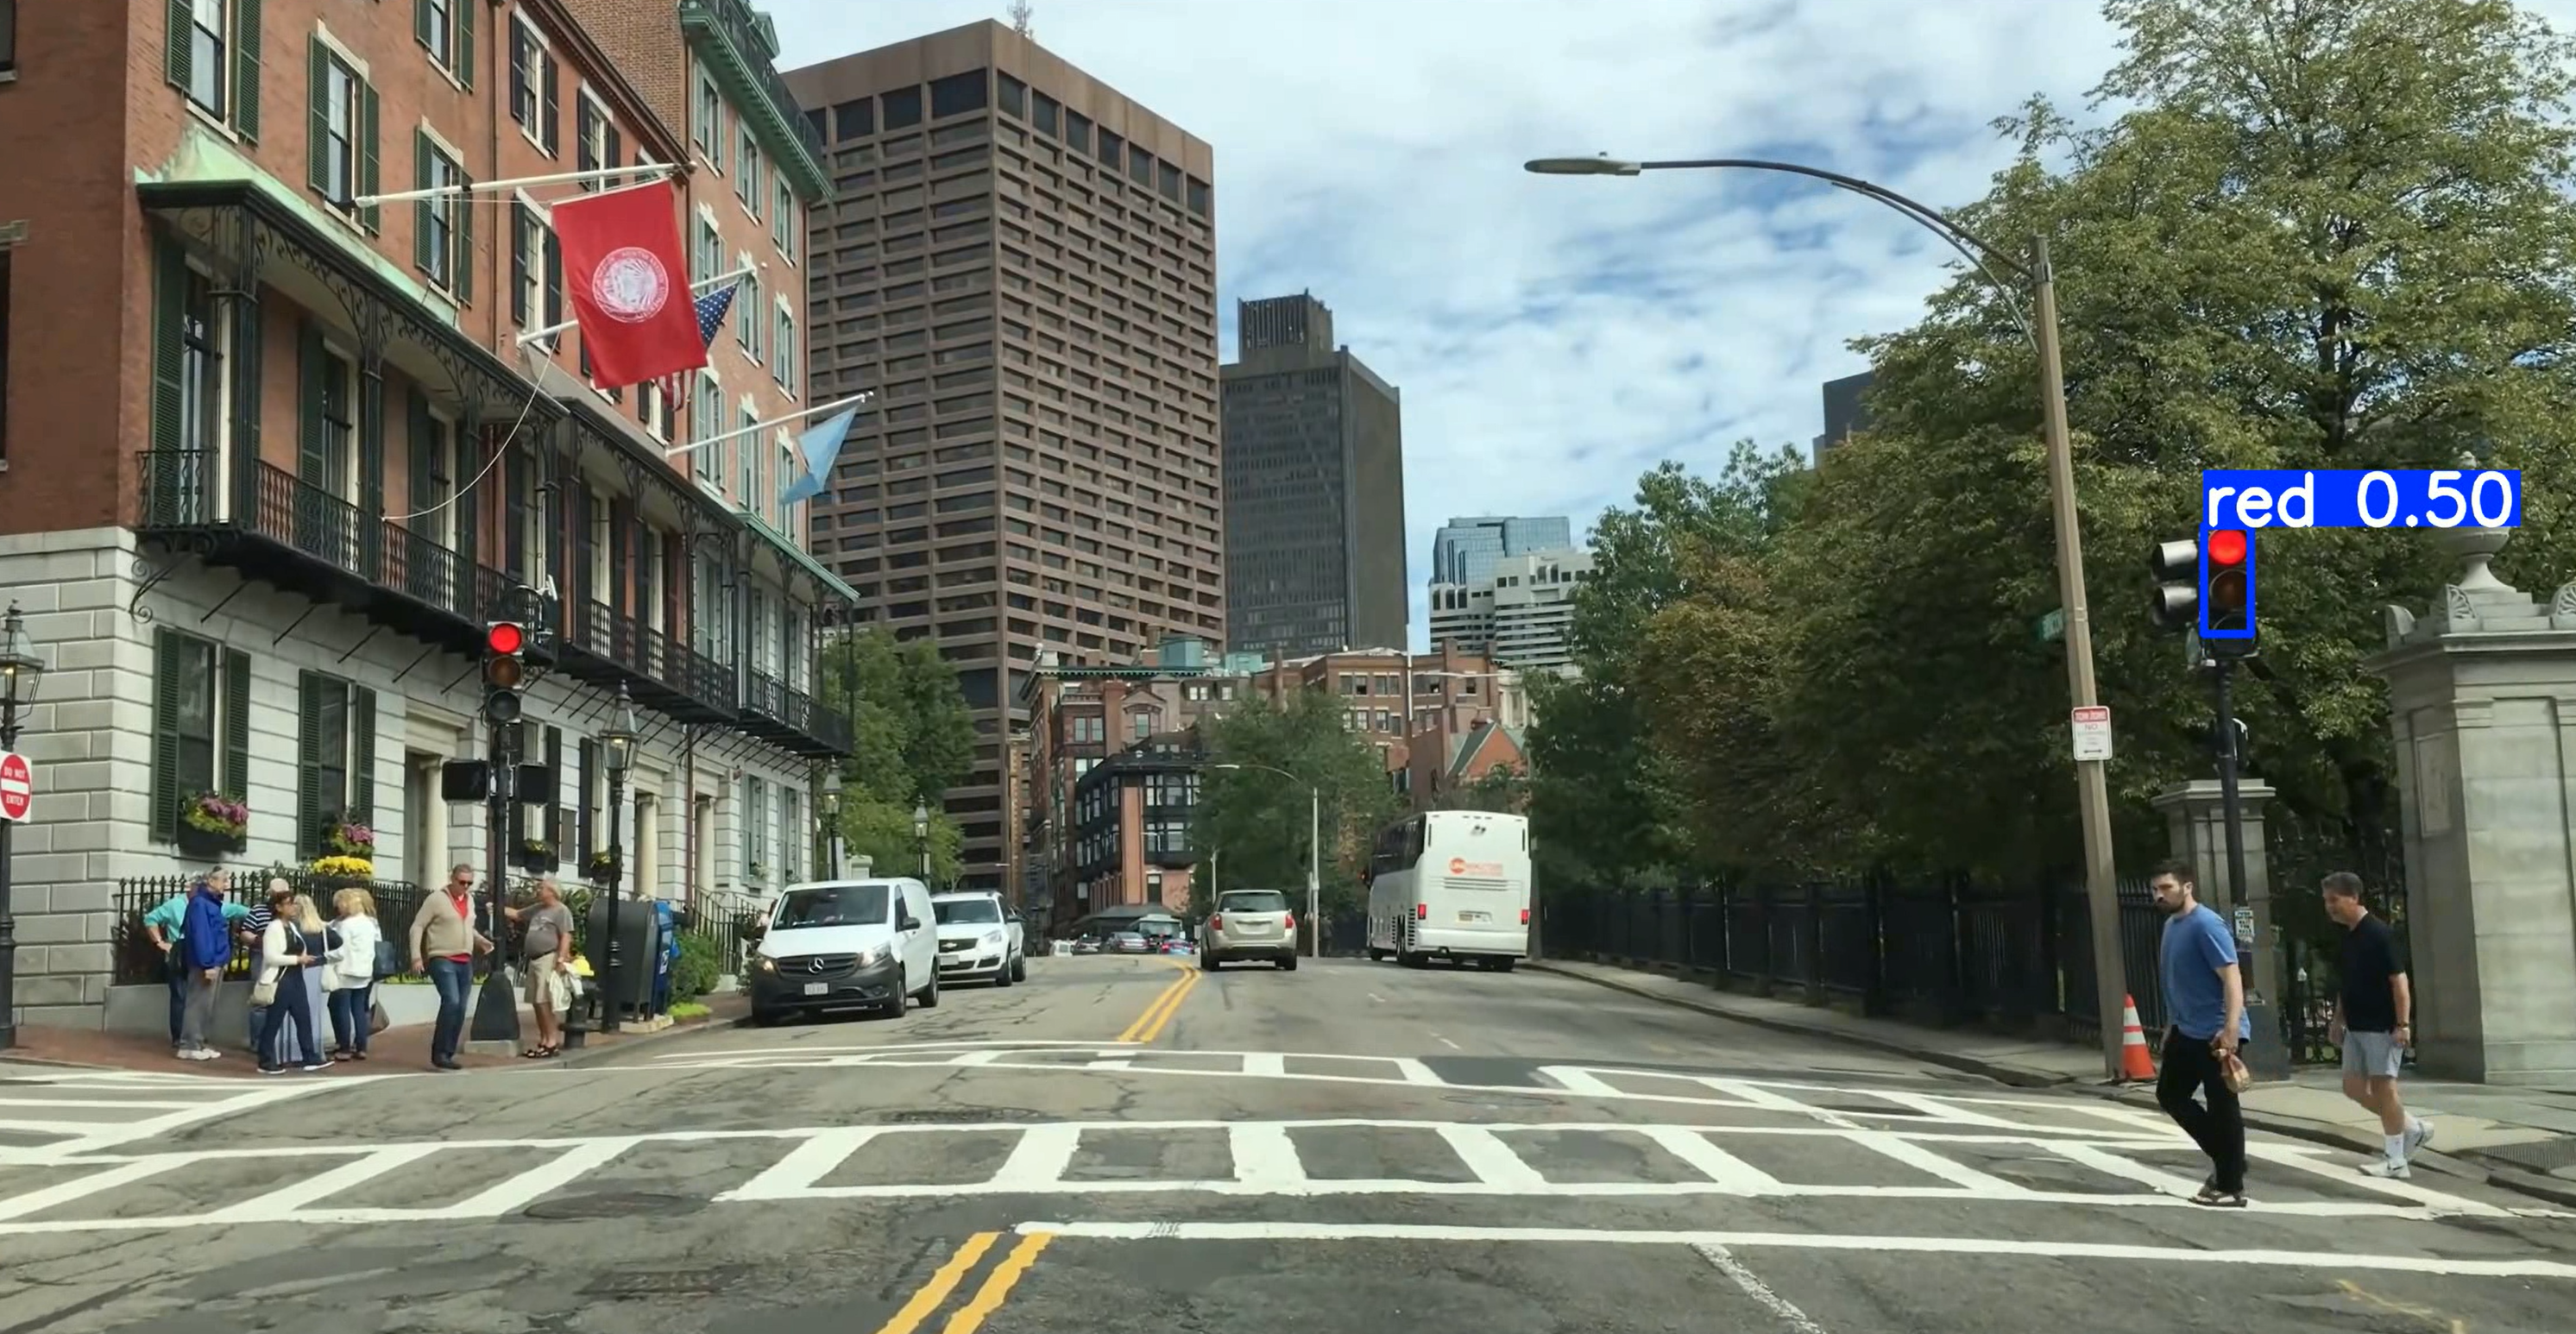
\includegraphics[width=\textwidth]{Video_Result_1.png}
        \caption{Performance of the mid-term model}
        \label{fig:Video_Result_1}
    \end{subfigure}
    \hfill
    \begin{subfigure}[b]{0.225\textwidth}
        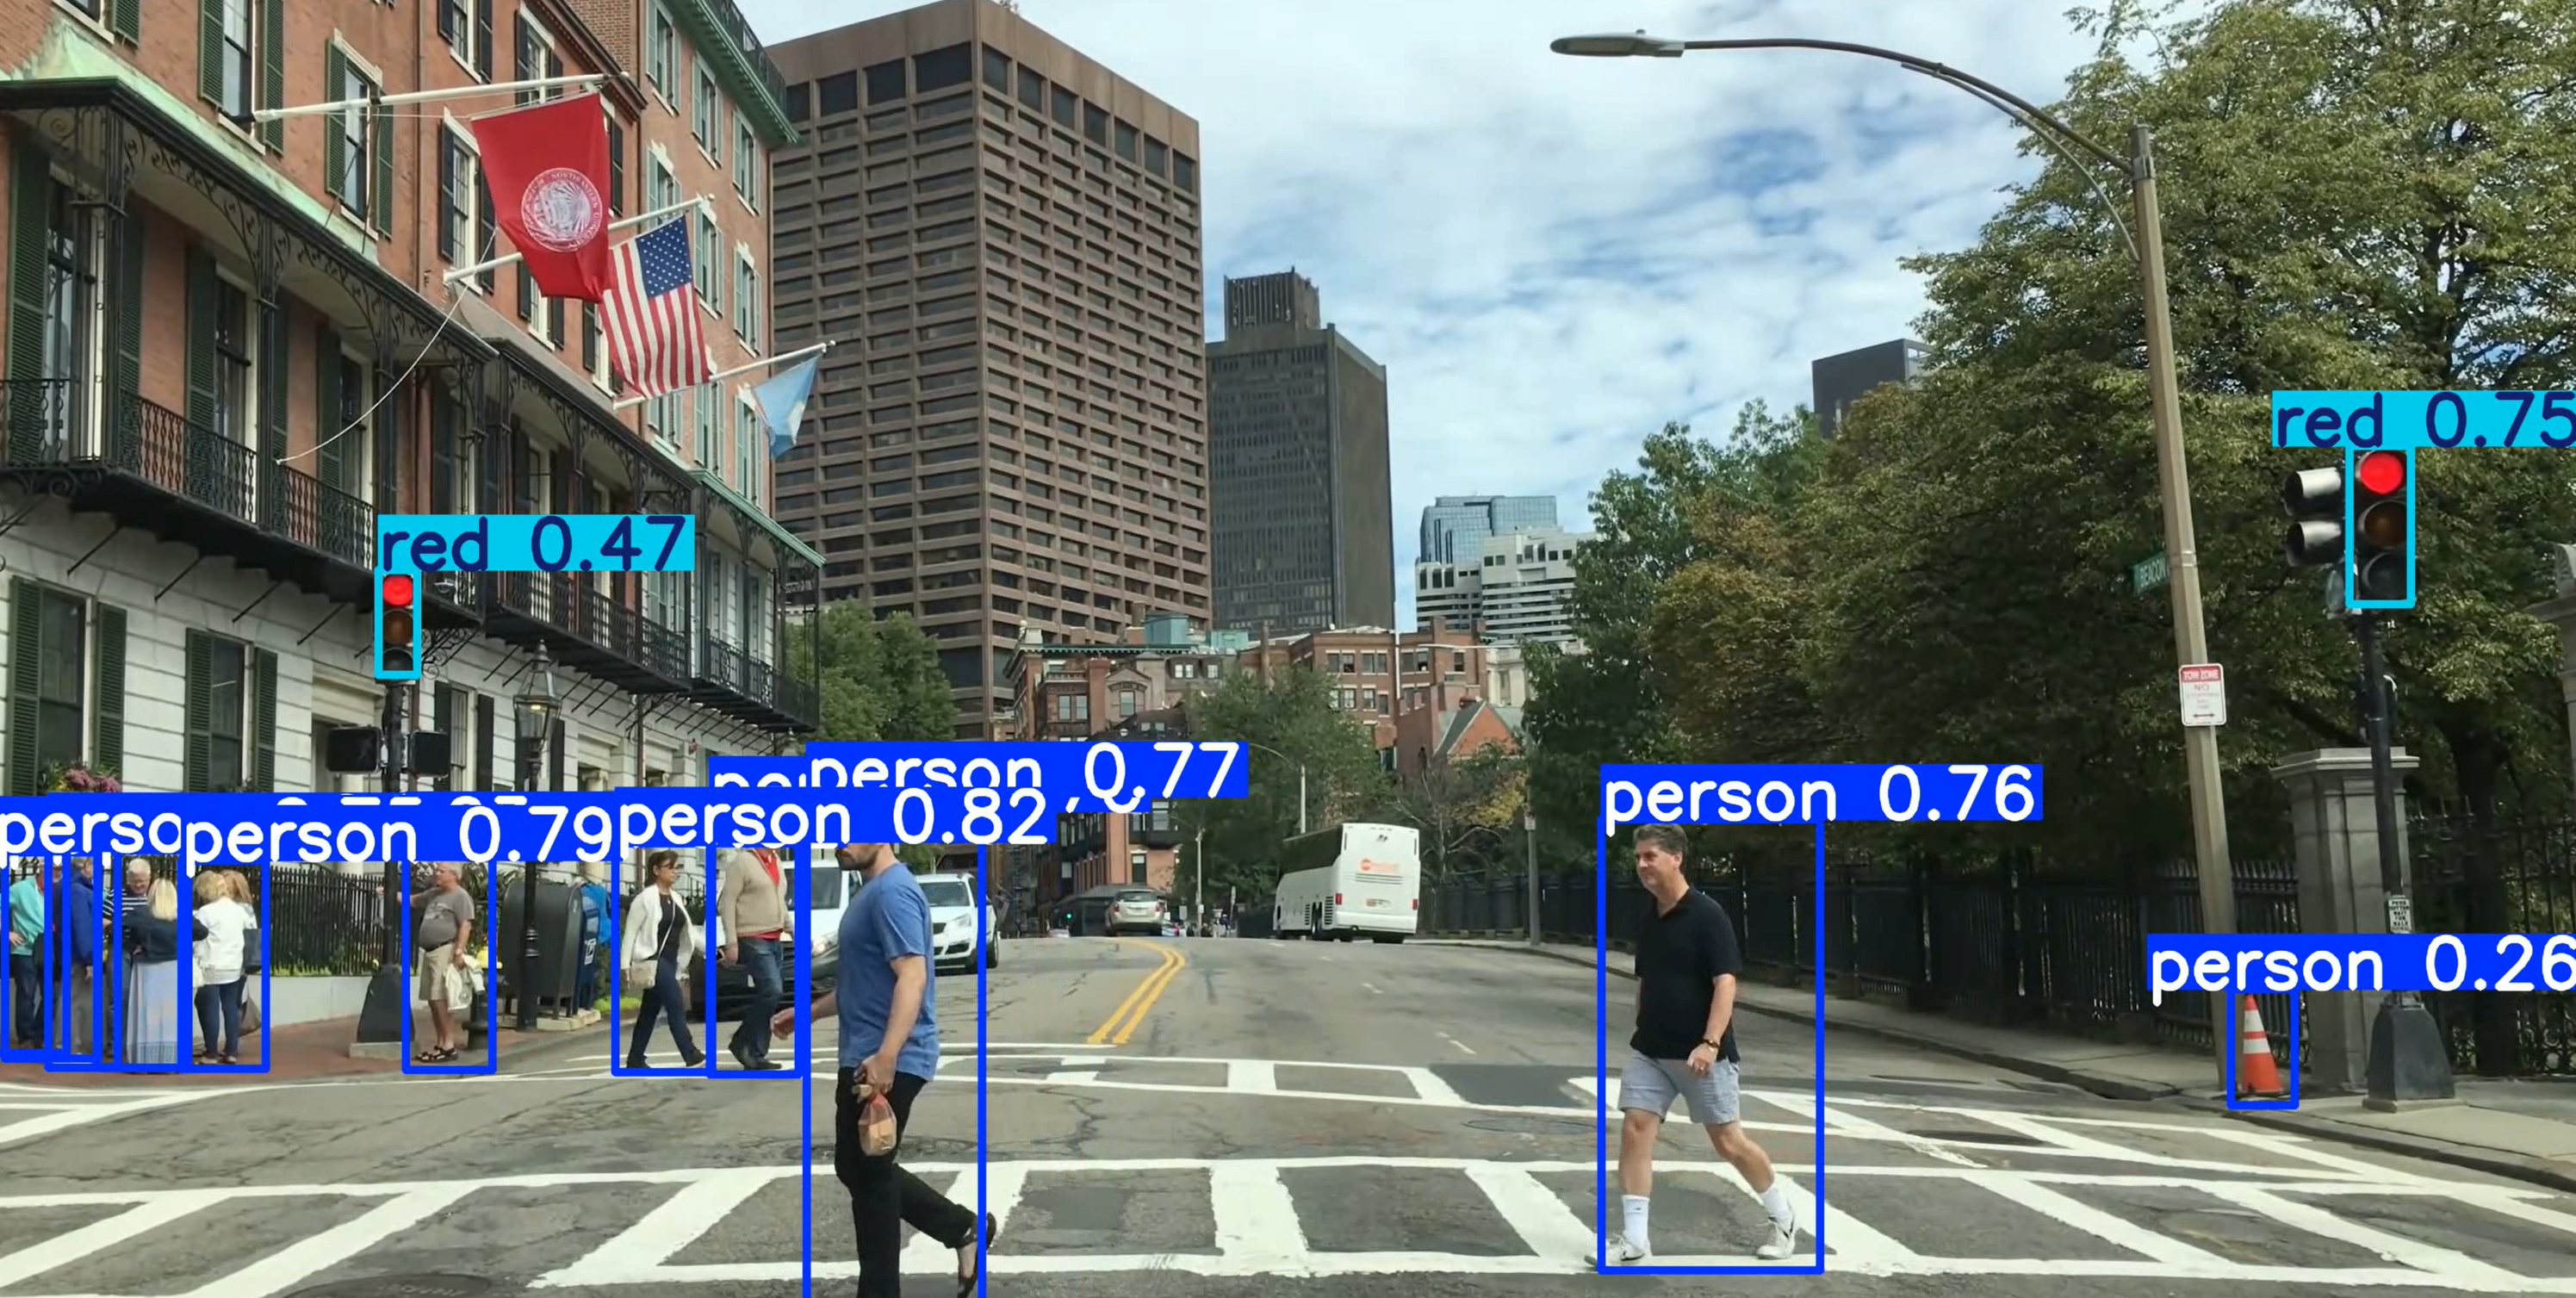
\includegraphics[width=\textwidth]{Video_Result_1_new.png}
        \caption{Performance of the current model
}
        \label{fig:Video_Result_1_new}
    \end{subfigure}
    \caption{Video Scenario 1}
    \label{fig:Video Scenario 1}
\end{figure}

ii. \textbf{Observed Limitations \& Failure Cases:}

As shown in Fig.~\ref{fig:Low Confidence Score}, when the vehicle nears the stop line, the current YOLOv8 model only marginally detects the traffic light on the right side, with a relatively low confidence score. The traffic light on the left, however, fails to be detected altogether. In practical applications, if the model identifies traffic lights only at such a late stage, the vehicle is left with insufficient reaction time, which could pose a serious safety hazard.

As shown in Fig.~\ref{fig:Object Confusion}, the current YOLOv8 model mistakenly identifies the flag at the top of the image as a stop sign. If an error-tolerant or correction mechanism is implemented without proper safeguards, the vehicle may interpret such false positives as valid inputs, potentially resulting in incorrect decisions and posing a significant safety risk.


\begin{figure}[h]
    \centering
    \begin{subfigure}[b]{0.25\textwidth}
        \includegraphics[width=\textwidth]{Video_Fail_Result_1.png}
        \caption{Low Confidence Score}
        \label{fig:Low Confidence Score}
    \end{subfigure}
    \hfill
    \begin{subfigure}[b]{0.25\textwidth}
        \includegraphics[width=\textwidth]{Video_Fail_Result_2.png}
        \caption{Object Confusion}
        \label{fig:Object Confusion}
    \end{subfigure}
    \caption{Failure Cases in Video Scenario}
    \label{fig:Failure Cases in Video Scenario}
\end{figure}

\subsection{Result of Real-time Recording Scenario}

The real-time recording scenario was taken in the parking lot at rice, as shown in Fig.~\ref{fig:Real-time Recording Scenario}, whose efficiency and limitations are similar to video one. 

\begin{figure}[h]
    \centering
    \includegraphics[width=0.25\textwidth]{Result_Real_Time_1.png}
    \caption{Real-time Recording Scenario}
    \label{fig:Real-time Recording Scenario}
\end{figure}

\section{Discussion}

Combined with the characteristics of the YOLOv8 algorithm, we summarize the following 3 main reasons leading to failure results.

i. \textbf{Unstable detection for near/far or occluded objects: } This can be attributed to YOLOv8's anchor-free, single-stage detection architecture, which still struggles with extreme scale variations. For solutions, we can integrate multi-scale feature enhancement modules such as BiFPN or Transformer-based FPN to improve sensitivity to extreme object sizes. Additionally, employ advanced data augmentation techniques like mosaic or random cropping to simulate occlusion scenarios.

ii. \textbf{Class confusion for visually similar objects: } This highlights the model’s insufficient representation capability for rare or long-tail classes, especially when training data is imbalanced. For solutions, we can introduce more hard negative samples for confusing classes and apply contrastive learning or class-aware attention modules to help the model better distinguish subtle differences in appearance.

iii. \textbf{Degraded performance under motion blur or low lighting in video frames: } This indicates the model’s sensitivity to temporal discontinuities and degraded image quality. For solutions, we can incorporate temporal modeling techniques (e.g., ConvLSTM or sliding-window fusion across frames) to capture temporal consistency. Also, apply image normalization or adaptive histogram equalization to address lighting variation.



\section{Future Work}

In future stages of development, we are going to focus on enhancing the performance and robustness of our object detection system. It can be divided into software module and hardware module according to Fig.~\ref{fig:The Structure of our Approach}

\subsection{Software Module}

i. \textbf{Enhancing the performance of Data Acquisition Part: }Future improvements include applying image preprocessing (e.g., enhancement, deblurring), expanding training data with diverse scenes, and optimizing real-time performance via pruning or hardware acceleration. To improve robustness, future models may adopt contrast-aware modules and multi-scale architectures for better detection under varied lighting and dense object conditions.



ii. \textbf{Build the basic structure of data processing and decision making parts: }The future goal is to establish core functionalities for the data processing and decision making modules. The data processing part should extract key features such as size, shape, color, and distance, using algorithms like OpenPose, Mask R-CNN, or MiDaS. The decision making module should analyze these features in real time to generate control commands (e.g., braking, acceleration, steering). Suitable techniques include finite state machines (FSM), reinforcement learning, and behavior cloning, ensuring timely and intelligent responses within the smart camera system.


\subsection{Hardware Module}

To validate the effectiveness of our software modules, we plan to implement the system on a commonly used model vehicle equipped with a USB camera, as shown in Fig.~\ref{fig:Some Hardware Module of Future Work}. This setup will allow us to conduct real-world testing of the object detection pipeline in dynamic environments. By integrating the trained model into the hardware platform, we aim to assess the system’s responsiveness, detection accuracy, and real-time performance under typical driving conditions.

\begin{figure}[h]
    \centering
    \begin{subfigure}[b]{0.225\textwidth}
        \includegraphics[width=\textwidth]{Model Car.jpeg}
        \caption{Vehicle Model}
        \label{fig:Model Car}
    \end{subfigure}
    \hfill
    \begin{subfigure}[b]{0.225\textwidth}
        \includegraphics[width=\textwidth]{Model Car Camera.jpeg}
        \caption{USB Camera}
        \label{fig:Model Car Camera}
    \end{subfigure}
    \caption{Some Hardware Module of Future Work}
    \label{fig:Some Hardware Module of Future Work}
\end{figure}



\clearpage
\twocolumn[
\begin{center}
    \section*{APPENDIX}
\end{center}
\vspace{0.5cm}
]
To support reproducibility and understanding, this appendix outlines the core logic of each implemented algorithm used in our smart camera system. Each algorithm aligns with a corresponding stage in the methodology or experiment section.
\vspace{-0.5em}

\begin{algorithm}[H]
\caption{Logic of Image Scenario Testing Code}
\begin{algorithmic}[1]
\STATE import YOLO model class from the \textit{ultralytics} package
\STATE import the \texttt{cv2} module
\STATE load trained model using weights \texttt{best.pt}
\STATE load target image from path \texttt{test.jpg}
\STATE perform object detection with confidence threshold = 0.25
\STATE extract annotated result from prediction output
\STATE display the annotated image in a pop-up window
\STATE wait for user input, then close the window
\end{algorithmic}
\end{algorithm}
\vspace{-5em}
This script demonstrates how the trained YOLOv8 model (\texttt{best.pt}) is used to perform object detection on static images. As described in Section III-C-i, it loads an image, applies the detection model with a defined confidence threshold, and visualizes annotated results. This serves to evaluate model performance across diverse image contexts.

\vspace{-0.5em}
\begin{algorithm}[H]
\caption{Logic of Video Scenario Testing Code}
\begin{algorithmic}[1]
\STATE import YOLO model class from the \textit{ultralytics} package
\STATE import the \texttt{cv2} module
\STATE load trained model from \texttt{best.pt}
\STATE open the camera device (0 for default, 1 for external)
\IF{camera fails to open}
    \STATE print error message and terminate
\ENDIF
\STATE create display window titled ``YOLO Realtime Detection''
\WHILE{camera is streaming frames}
    \STATE read a frame from the camera
    \IF{frame read fails}
        \STATE print failure message and break loop
    \ENDIF
    \STATE perform detection on the frame using the model ({conf = 0.25})
    \STATE retrieve and visualize detection results
    \STATE show annotated frame in display window
    \IF{key 'q' is pressed}
        \STATE break loop and exit
    \ENDIF
\ENDWHILE
\STATE release camera and destroy all windows
\end{algorithmic}
\end{algorithm}
\vspace{-5em}
Used in Section III-C-ii, this code applies YOLOv8 to video streams. It opens a video file or live camera feed, processes each frame for object detection, and displays the results in real-time. This helps test the model's robustness under continuous, dynamic visual inputs such as dashcam footage.
\vspace{13em}

\begin{algorithm}[H]
\caption{Logic of Real-time Recording Scenario Testing Code}
\begin{algorithmic}[1]
\STATE import YOLO model class from the \textit{ultralytics} package
\STATE import \texttt{cv2} for video stream handling
\STATE load trained model from \texttt{best.pt}
\STATE open external camera using \texttt{cv2.VideoCapture(1)}
\IF{camera fails to open}
    \STATE print error message and exit the script
\ENDIF
\STATE create a window named {"YOLO Realtime Detection"}
\WHILE{camera is streaming frames}
    \STATE read a frame from the camera
    \IF{frame read fails}
        \STATE print failure message and break the loop
    \ENDIF
    \STATE perform object detection on the frame with confidence threshold = 0.25
    \STATE plot the detection results onto the frame
    \STATE display the annotated frame in the window
    \IF{key 'q' is pressed}
        \STATE break the loop
    \ENDIF
\ENDWHILE
\STATE release camera and close all windows
\end{algorithmic}
\end{algorithm}
\vspace{-1em}
As mentioned in Section III-C-iii, this script connects to an external USB camera and performs real-time detection on live video. It demonstrates the system’s responsiveness and deployment feasibility in real-world scenarios, capturing frames and running inference continuously.
\vspace{2em}
\begin{algorithm}[H]
\caption{Logic of YOLOv8 Training Script}
\begin{algorithmic}[1]
\STATE import YOLO model class from the \textit{ultralytics} package
\IF{this script is executed as the main program}
    \STATE initialize model with pre-trained weights \textit{yolov8n.pt}
    \STATE start model training with the following settings:
    \STATE \hspace{1em} - dataset defined in \textit{Dataset/data.yaml}
    \STATE \hspace{1em} - use GPU device 0
    \STATE \hspace{1em} - train for 50 epochs
\ENDIF
\end{algorithmic}
\end{algorithm}
\vspace{-1em}
This script, detailed in Section III-B-ii, trains the YOLOv8 model using either open-source or custom datasets. It leverages the Ultralytics library, initializes from a pre-trained model, and references the \texttt{data.yaml} configuration. It outputs weight files like \texttt{best.pt}, which are then used in subsequent experiments.

% Can use something like this to put references on a page
% by themselves when using endfloat and the captionsoff option.
\ifCLASSOPTIONcaptionsoff
  \newpage
\fi



% trigger a \newpage just before the given reference
% number - used to balance the columns on the last page
% adjust value as needed - may need to be readjusted if
% the document is modified later
%\IEEEtriggeratref{8}
% The "triggered" command can be changed if desired:
%\IEEEtriggercmd{\enlargethispage{-5in}}

% references section

% can use a bibliography generated by BibTeX as a .bbl file
% BibTeX documentation can be easily obtained at:
% http://mirror.ctan.org/biblio/bibtex/contrib/doc/
% The IEEEtran BibTeX style support page is at:
% http://www.michaelshell.org/tex/ieeetran/bibtex/
%\bibliographystyle{IEEEtran}
% argument is your BibTeX string definitions and bibliography database(s)
%\bibliography{IEEEabrv,../bib/paper}
%
% <OR> manually copy in the resultant .bbl file
% set second argument of \begin to the number of references
% (used to reserve space for the reference number labels box)
\clearpage

\section*{Acknowledgment}
The authors would like to thank KTM Technology for sponsoring this Smart Camera project for the ELEC 594 program.

\begin{thebibliography}{1}

\bibitem{SelfDriving}
S. Santosh Kumar, \emph{Self-Driving Car Using Neural Networks and
Computer Vision}\hskip 1em plus
  0.5em minus 0.4em\relax IEEE ,IIHC, 2022.


\bibitem{Controlling Mobile Robot}
Khansaa Dheyaa Ismael, \emph{Controlling Mobile Robot Navigation Equipped with Computer Vision Perception for Text using OCR
Technique}\hskip 1em plus
 0.5em minus 0.4em\relax IEEE, SSD, 2024.

 \bibitem{Smart Cameras}
David Brady, \emph{Smart Cameras}\hskip 1em plus
 0.5em minus 0.4em\relax  Duke university, 2020.

\bibitem{Design and Realization}
Xuanxuan Hong, \emph{Design and Realization of Fire Detection Using
Computer Vision Technology}\hskip 1em plus
 0.5em minus 0.4em\relax  IEEE, CCDC, 2019

\bibitem{Camera-trap-classifier}
Macro-willi, \emph{Camera-trap-classifier}\hskip 1em plus
 0.5em minus 0.4em\relax  GitHub repository, 2019.
[Online]

\bibitem{UniScene}
Chaytonmin, \emph{UniScene}\hskip 1em plus
 0.5em minus 0.4em\relax  GitHub repository, 2023.
[Online]

\bibitem{Autodrone}
MECE students, \emph{Autodrone}\hskip 1em plus
 0.5em minus 0.4em\relax  Rice Unv. ,GitHub repository, 2024.
[Online]

\bibitem{fasterrcnn}
S.~Ren, K.~He, R.~Girshick, and J.~Sun, \emph{Faster R-CNN: Towards Real-Time Object Detection with Region Proposal Networks}\hskip 1em plus 0.5em minus 0.4em\relax arXiv preprint arXiv:1506.02640, 2015. [Online]. Available: \url{https://arxiv.org/abs/1506.02640}

% \bibitem{FSD}
% Tesla, \emph{Autopilot and Full Self-Driving (Supervised)}\hskip 1em plus 0.5em minus 0.4em\relax Tesla

% \bibitem{Autopilot}
% K. Nived Maanyu, \emph{A Study on Tesla Autopilot}\hskip 1em plus 0.5em minus 0.4em\relax Sreenidhi Institute of Science And Technology, 2020 

% \bibitem{ExSolution}
% Syazvinski, \emph{Traffic-Light-Detection-Color-Classification}\hskip 1em plus
% 0.5em minus 0.4em\relax GitHub repository, 2023.
% [Online]

% \bibitem[Fig.4]
% *Carousel, \emph{Manderfield Highway Information}\hskip 1em plus 0.5em minus 0.4em\relax Beaver County, 2024

% \bibitem[Fig.5-(a)]
% *Kidloverz22, \emph{Seoul,South Korea-March 2019: Close up image of traffic light changes color with Korean traffic street sign}\hskip 1em plus 0.5em minus 0.4em\relax Dreamstime.com

% \bibitem[Fig.5-(b)]
% *Katherine Tweed, \emph{Better Traffic Light Simulations Could Cut Travel Time and Gas Use}c IEEE Spectrum, 2014
% \bibitem[Fig.5-(c)]
% *Ben Watanabe, \emph{Those blue lights on traffic signals help nab red-light runners}\hskip 1em plus 0.5em minus 0.4em\relax HeraldNet, 2022

\end{thebibliography}



% biography section
% 
% If you have an EPS/PDF photo (graphicx package needed) extra braces are
% needed around the contents of the optional argument to biography to prevent
% the LaTeX parser from getting confused when it sees the complicated
% \includegraphics command within an optional argument. (You could create
% your own custom macro containing the \includegraphics command to make things
% simpler here.)
%\begin{IEEEbiography}[{\includegraphics[width=1in,height=1.25in,clip,keepaspectratio]{mshell}}]{Michael Shell}
% or if you just want to reserve a space for a photo:


% insert where needed to balance the two columns on the last page with
% biographies
%\newpage


% You can push biographies down or up by placing
% a \vfill before or after them. The appropriate
% use of \vfill depends on what kind of text is
% on the last page and whether or not the columns
% are being equalized.

%\vfill

% Can be used to pull up biographies so that the bottom of the last one
% is flush with the other column.
%\enlargethispage{-5in}



% that's all folks
\end{document}


